En una actividad del colegio, se diseña una figura decorativa formada por un rectángulo y dos semicírculos: uno en la parte superior (agregado) y otro en la parte inferior (recortado). La figura tiene un ancho de 4 cm y una altura de 6 cm. Ambos semicírculos tienen como diámetro el ancho del rectángulo.

\begin{center}
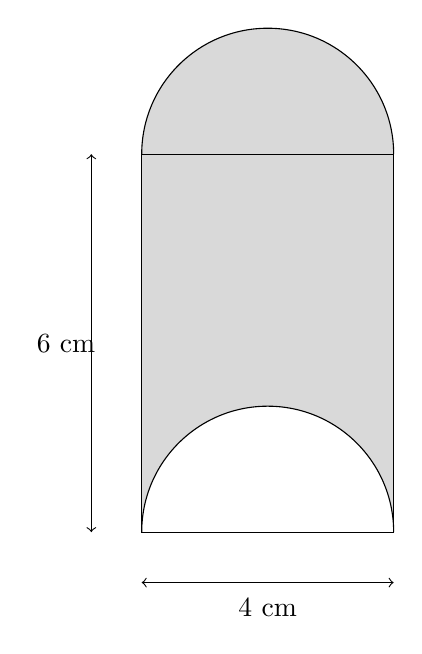
\begin{tikzpicture}[scale=0.8]

% Área sombreada (construcción correcta)
\fill[gray!30]
(0,0) -- (0,6)
-- (0,6) arc[start angle=180,end angle=0,radius=2]
-- (4,6) -- (4,0)
-- (4,0) arc[start angle=0,end angle=180,radius=2]
-- cycle;

% Bordes
\draw (0,0) rectangle (4,6);
\draw (0,6) arc[start angle=180,end angle=0,radius=2];
\draw (4,0) arc[start angle=0,end angle=180,radius=2];

% Medidas
\draw[<->] (0,-0.8) -- (4,-0.8);
\node at (2,-1.2) {4 cm};

\draw[<->] (-0.8,0) -- (-0.8,6);
\node at (-1.2,3) {6 cm};

\end{tikzpicture}
\end{center}

¿Cuál es el área de la figura sombreada?

\begin{multicols}{2}
\begin{enumerate}[label=\alph*), leftmargin=*]
\item $24$
\item $24 + 2\pi$
\item $24 - 2\pi$
\item $24 + \pi$
\end{enumerate}
\end{multicols}